\section{Results}
This section will show what kind of setup was used to test the performances of our implementations and what results were achieved.

\subsection{Expected results}
First of all\textbf{ I expected the completion times of both implementations to be somewhat similar} given their same structure, this implies that they will also have some \textbf{similarity on their speedup and others metrics}.
\vspace{3mm}

Speaking about the speedup, we know that it is equal to $\frac{T_{seq}}{T_{par(nw)}}$ and that the ideal one is exactly the parallelism degree, $nw$; this means that, in a real world environment, the achievable speedup is $s(nw)<nw$, let's check it this fact holds:
\begin{center}
\begin{Large}
$s(nw)=\frac{T_{seq}}{T_{par}}=\frac{T_{Read}+n(T_{knn}+T_{BuildString})+T_{Write}}{T_{Read}+nwT_{ov}+\frac{n(T_{knn}+T_{BuildString})}{nw}+T_{Write}}$
\end{Large}
\end{center}
It is safe to assume that $T_{Read}$ and $T_{Write}$ are negligible with respect to the total completion time so everything reduces to:
\begin{center}
\begin{Large}
$s(nw)=\frac{n(T_{knn}+T_{BuildString})}{nwT_{ov}+\frac{n(T_{knn}+T_{BuildString})}{nw}}$
\end{Large}
\end{center}
And this is surely less than $nw$ as we know from the lectures.

\subsection{Setup}
Before we talk about the results I decided that it was necessary to explain some choices beforehand:
\begin{itemize}
    \item The results were all obtained on the \textbf{64-core with four-way hyperthreading Intel XEON-PHI}.
    \item For each configuration \textbf{I did not take into consideration $T_{Read}$, $T_{Write}$ and $T_{ov}$} since they were nearly the same for each configuration with the same amount of points, moreover the most interesting part is the \textit{non-serial} one, which is $n(T_{knn}+T_{BuildString})$.
    \item \textbf{Each configuration was run ten times}.
    \item The\textbf{ chosen value for k was 10 for all the configuration}, hence all the results in the next subsections are averages.
    \item The \textbf{parallelism degree was decided to be $2^i$} where $i\in\{0, .., 8\}$.
    \item \textbf{Times were obtained using the utimer class} that the professor showed during the lectures.
\end{itemize}
\subsection{Results on the XEON-PHI machine}
I decided to run tests on 2d spaces with \textbf{10k, 20k, 50k and 100k points} where every point was drawn by an uniform distribution over [0, 10]; the number of points was decided as such in order to see \textbf{how each implementation perform going from a sparse spaces to densely populated ones}. First of all it was necessary to calculate the amount of time spent by the execution of the sequential knn version in order to get values needed to obtain the other metrics (e.g.: speedup and efficiency), \autoref{table:knn_sequential_results} shows the results achieved by such implementation.

\begin{table}[H]
\centering
\begin{tabular}{c|c|c|c}\hline \hline
\multicolumn{4}{c}{\textbf{Sequential 10-KNN execution times ($\mu$sec)}} \\\hline
\textbf{10k points} & \textbf{20k points} & \textbf{50k points} & \textbf{100k points}\\\hline
4187051 & 15973321 & 95360616 & 375058248 \\
\hline \hline
\end{tabular}
\caption{Results with the sequential implementation.}
\label{table:knn_sequential_results}
\end{table}
As one would expect, the time does not scale linearly with the number of points since the cost of \autoref{algorithm:knn} is $O(n^2log(k))$, something more interesting arose during the execution of C++ threads and FastFlow versions whose results are shown in \autoref{table:knn_parallel_fastflow_results}.

\begin{table}[H]
\centering
\begin{tabular}{c||c|c|c|c||c|c|c|c}\hline \hline
\multicolumn{9}{c}{\textbf{Parallel and FastFlow 10-KNN execution times ($\mu$sec)}} \\\hline \hline
\multirow{2}{*}{\textbf{nw}} & \multicolumn{4}{c||}{\textbf{stdlib threads}} & \multicolumn{4}{c}{\textbf{FastFlow}} \\\cline{2-9}
& \textbf{10k} & \textbf{20k} & \textbf{50k} & \textbf{100k} & \textbf{10k} & \textbf{20k} & \textbf{50k} & \textbf{100k} \\\hline
1 & 4195076 & 16573213 & 98816008 & 377017508 & 4198343 & 15989082 & 96277045 & 406293436 \\
2 & 2150114 & 8006220 & 50251728 & 201949754 & 2124308 & 8018496 & 48329593 & 201459406 \\
4 & 1324868 & 4072286 & 27676599 & 99481003 & 1072248 & 4034389 & 2422181 & 99968804 \\
8 & 726914 & 2030168 & 13578018 & 51113708 & 539050 & 2021035 & 12098202 & 50136748 \\
16 & 322046 & 1087086 & 6741971 & 24312895 & 316082 & 1062674 & 6183317 & 26882276 \\
32 & 182296 & 677542 & 3472759 & 14382776 & 210621 & 588005 & 3461644 & 14591443 \\
64 & 133958 & 434134 & 2151317 & 8876960 & 141363 & 400733 & 2278688 & 9016368 \\
128 & 99786 & 308973 & 1590471 & 6123643 & 106730 & 318886 & 1665072 & 6326216 \\
256 & 99371 & 256716 & 1046949 & 3969818 & 95743 & 274393 & 1122244 & 4312146 \\ \hline \hline
\end{tabular}
\caption{Results with the stdlib threads and FastFlow implementations.}
\label{table:knn_parallel_fastflow_results}
\end{table}

\subsection{Results analysis}
As first thing I want to underline is the fact that \textbf{the results are extremely similar between the two implementations} since, as I said in \autoref{subsec:par_implementations}, the two versions are basically the same with some minor changes.

\subsubsection{Execution times}
The execution times comparison (only for 50k and 100k points) is shown in \autoref{fig:results}
\begin{figure}[H]
    \centering
    \subfloat[C++ threads]{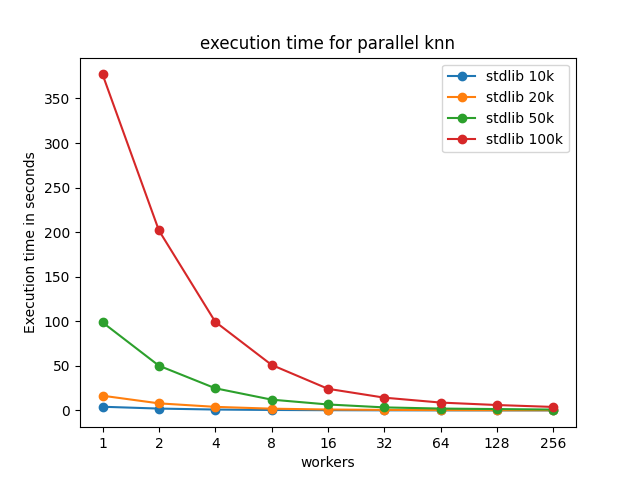
\includegraphics[width=0.45\linewidth]{images/knn_parallel_results.png}}
    \subfloat[FastFlow]{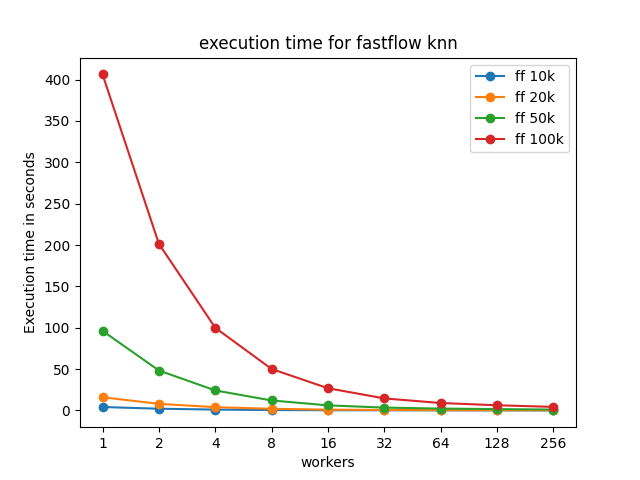
\includegraphics[width=0.45\linewidth]{images/knn_fastflow_results.png}}\\
    \subfloat[Comparison]{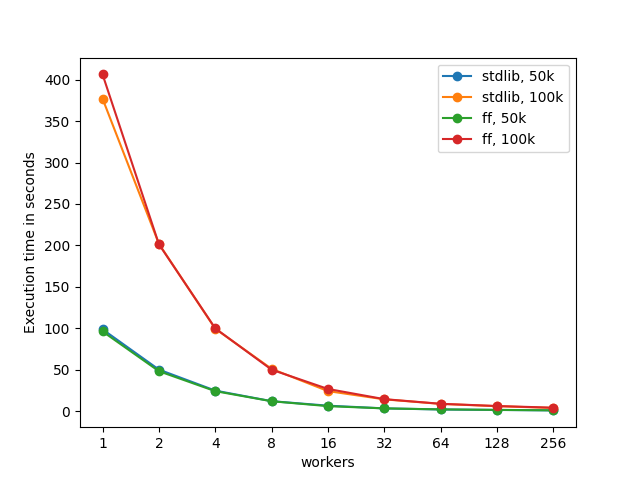
\includegraphics[width=0.45\linewidth]{images/knn_comparison_results.png}}
    \caption{Execution times for C++ threads and FastFlow versions and their comparison}
    \label{fig:results}
\end{figure}

\subsubsection{Speedup}
Let's now see and compare the speedup obtained by both implementations as shown in \autoref{fig:speedup}
\begin{figure}[H]
    \centering
    \subfloat[C++ threads]{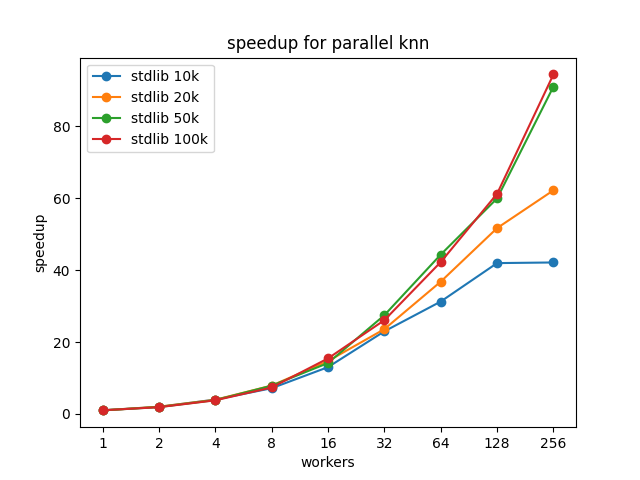
\includegraphics[width=0.45\linewidth]{images/knn_parallel_speedup.png}}
    \subfloat[FastFlow]{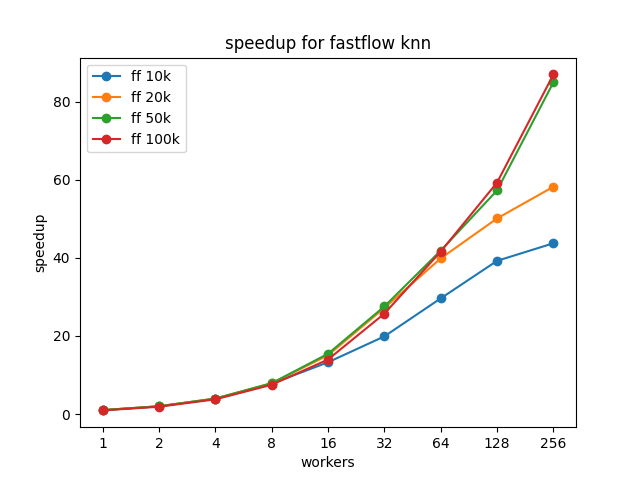
\includegraphics[width=0.45\linewidth]{images/knn_fastflow_speedup.png}}\\
    \subfloat[Comparison]{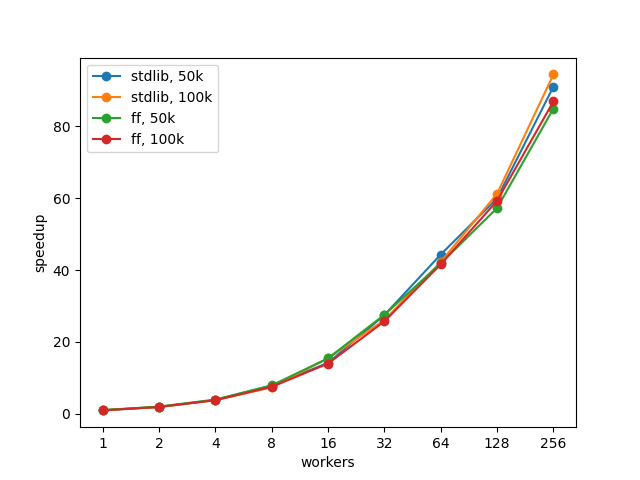
\includegraphics[width=0.45\linewidth]{images/knn_comparison_speedup.png}}
    \caption{Speedup for C++ threads and FastFlow versions and their comparison}
    \label{fig:speedup}
\end{figure}
The \textbf{speedup seems to scale well with the number of workers as long the number of points goes up}, in fact I could clearly see that for sparse 2d spaces (e.g.: 10k and 20k points) \textbf{the speedup seemed to reach a sort of plateau} the more I increased $nw$.
\vspace{3mm}

Since the execution times are the same \textbf{it was natural that the two versions would have similar speedup}, this will be the same for the next metrics that we are going to see.
\subsubsection{Scalability}
Scalability is the ratio between the parallel execution time with parallelism degree equal to 1 and the parallel execution with parallelism degree equal to $nw$, the ideal value is the same as for the speedup ($nw$).
\begin{center}
\begin{Large}
$scalab(nw)=\frac{T_{par}(1)}{T_{par(nw)}}$
\end{Large}
\end{center}
It measures how the parallel implementation achieves efficiently better performance the more the parallelism degree increases.
\begin{figure}[H]
    \centering
    \subfloat[C++ threads]{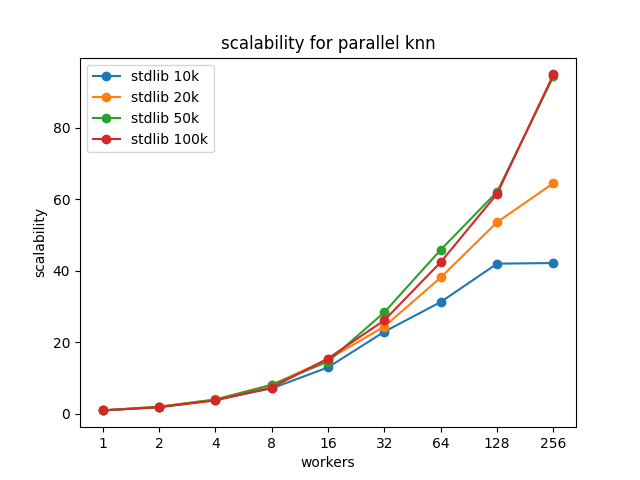
\includegraphics[width=0.45\linewidth]{images/knn_parallel_scalability.png}}
    \subfloat[FastFlow]{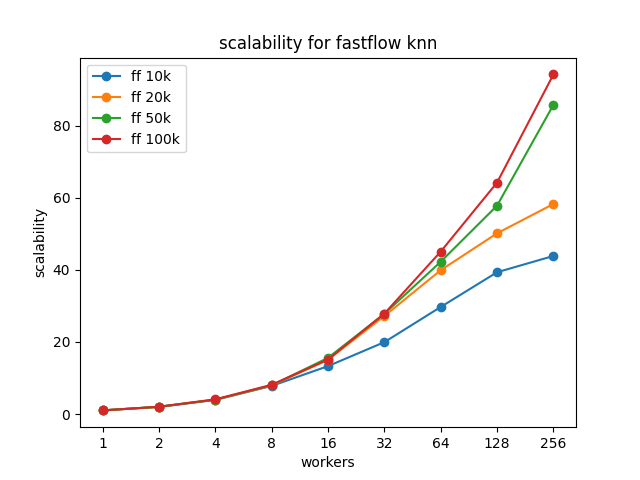
\includegraphics[width=0.45\linewidth]{images/knn_fastflow_scalability.png}}\\
    \subfloat[Comparison]{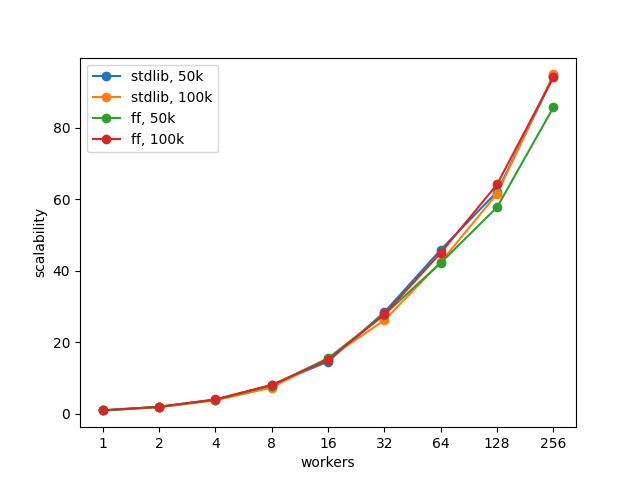
\includegraphics[width=0.45\linewidth]{images/knn_comparison_scalability.png}}
    \caption{Scalability for C++ threads and FastFlow versions and their comparison}
    \label{fig:scalability}
\end{figure}
What we have discussed briefly during the speedup analysis holds for the scalability too.

\subsubsection{Efficiency}
As last metric of the analysis it was natural to choose efficiency which is the ratio between the ideal execution time and the actual execution time.
\begin{center}
\begin{Large}
$\epsilon(nw)=\frac{T_{id}(nw)}{T_{par}(nw)}=\frac{T_{seq}}{nwT_{par}(nw)}=\frac{s(nw)}{nw}$
\end{Large}
\end{center}
The formula holds since $T_{id}=\frac{T_{seq}}{nw}$, moreover \textbf{efficiency measures how a parallel implementation is making use of the available resources}. The ideal value for the efficiency is 1 given the fact that the speedup is bound by $nw$.
\begin{figure}[H]
    \centering
    \subfloat[C++ threads]{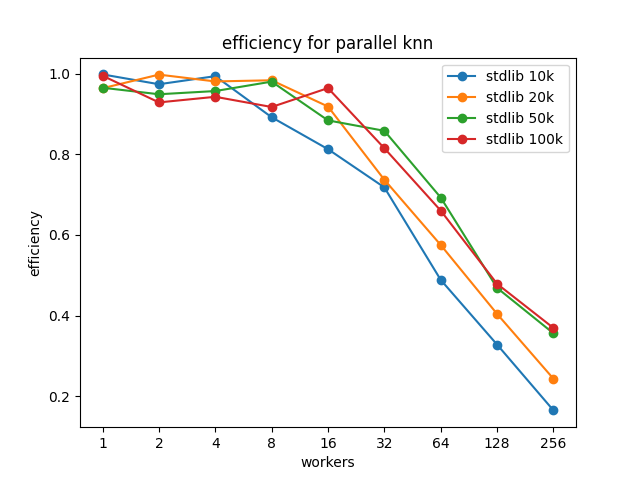
\includegraphics[width=0.45\linewidth]{images/knn_parallel_efficiency.png}}
    \subfloat[FastFlow]{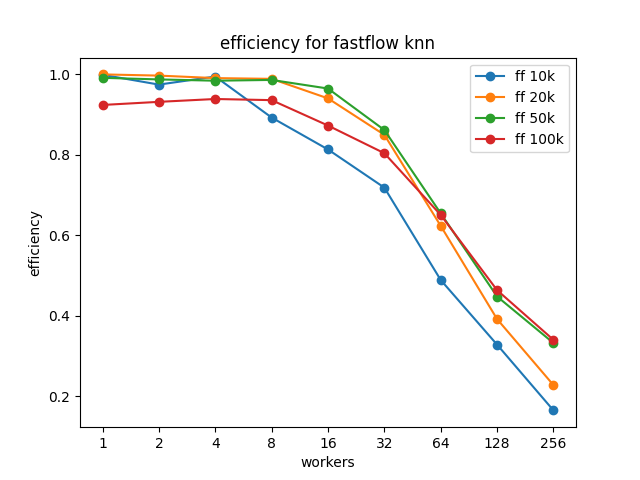
\includegraphics[width=0.45\linewidth]{images/knn_fastflow_efficiency.png}}\\
    \subfloat[Comparison]{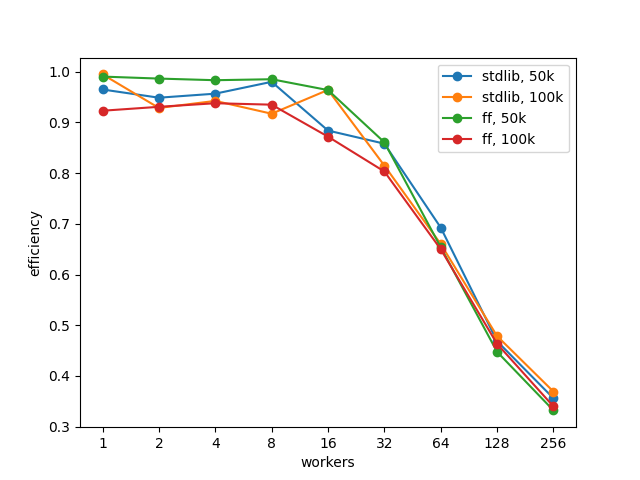
\includegraphics[width=0.45\linewidth]{images/knn_comparison_efficiency.png}}
    \caption{Efficiency for C++ threads and FastFlow versions and their comparison}
    \label{fig:efficiency}
\end{figure}
The most interesting thing is the fact that the efficiency has a strange plot from 2 to 16 workers as shown in \autoref{fig:efficiency}, this could be caused by the congestion on the XEON-PHI machine from other students while I was working on it (but I do not want to blame them as everyone needs to do project) or by routine tasks of the machine itself.
\vspace{3mm}

Another thing is the fact that \textbf{configurations with more points had a better efficiency than the ones working on sparse spaces}, but this comes to no surprise since the former had an higher speedup than the latter.